
\subsection{Systemarchitektur}

Dieses Kapitel beschreibt die Komponenten des Praxisrufsystems und wie diese erweitert werden.
Das System wird um Komponenten zur Signalvermittlung und Sprachsynthese erweitert.
Weiter wird die interne Struktur des Cloudservices angepasst um die Weiterentwicklung und Betrieb des Systems zu vereinfachen.

\begin{figure}[h]
    \centering
    \begin{minipage}[b]{0.8\textwidth}
        \fbox{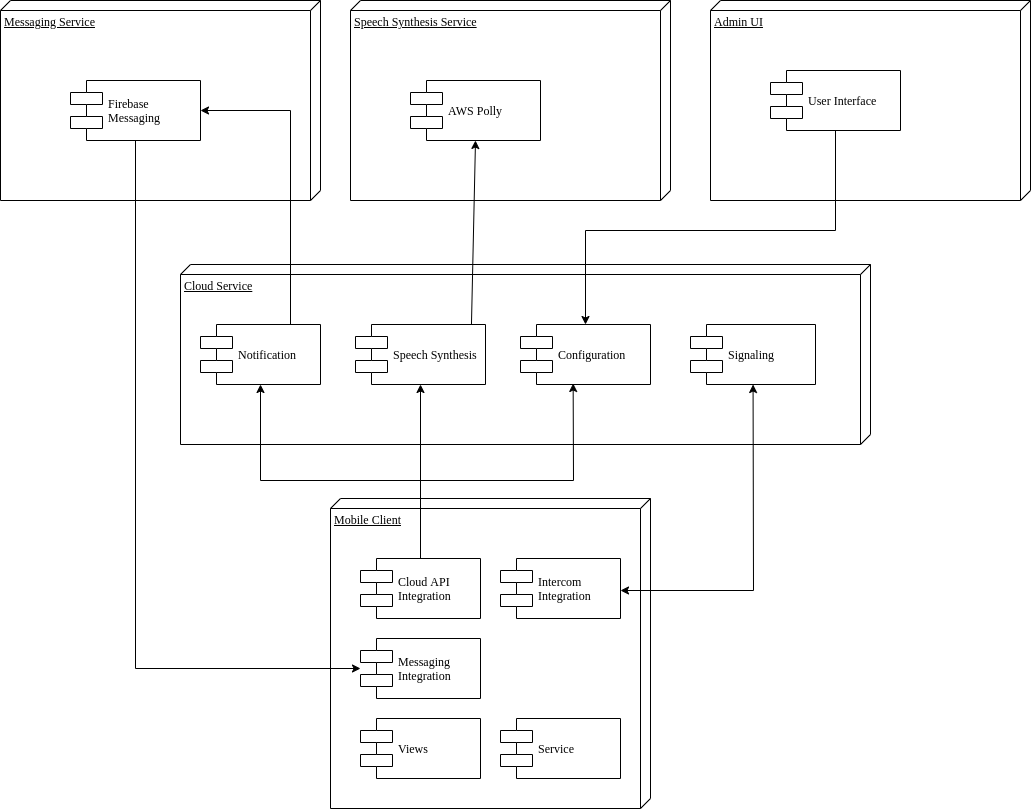
\includegraphics[width=\textwidth]{graphics/diagramms/Component_System_V02}}
        \caption{Systemkomponenten}
    \end{minipage}
\end{figure}

Abbildung 7.1 gibt einen Überblick über die Systemkomponenten und welche Teile diese beinhalten.
Die Pfeile zwischen Komponenten zeigen gerichtete Abfragen und damit eine Funktionale Abhängigkeit.
Alle dargestellten Komponenten sind entkoppelt und Abfragen finden nur über definierte Schnittstellen statt.

\subsubsection{Systemkomponenten}

Dieses Kapitel beschreibt die in Abbildung 7.1 abgebildeten Systemkomponenten.
Dabei wird für jede Komponente beschrieben, welche Aufgaben ihr zufallen und wie sie im Rahmen dieses Projektes erweitert wird.

\textbf{Cloudservice}

Der Cloudservice bildet das zentrale Serverkomponente des Praxisrufsystems.
Zu Beginn dieses Projektes umfasst der Cloudservice die beiden Domänen Notification und Configuration.
Dabei ist die Domäne Notification für das Versenden von Benachrichtigungen und die Domäne Configuration für die Verwaltung und Auswertung der Konfigurationen verantwortlich.
Die relevanten Empfänger für eine Benachrichtigung werden in der Configuration Domain ermittelt.
Um auf diese Informationen zugreifen zu können, muss aus der Notification Domain eine Abfrage an die Configuration Domain geschehen.
Die Configuration Domäne bietet dazu eine REST Schnittstelle~\cite{ip5}.

Die Trennung der Domänen wurde im Vorgängerprojekt lediglich auf Package-Ebene realisiert.
Mit diesem Projekt soll die Trennung einen Schritt weiter gehen.
Der Cloudservice wird Module aufgeteilt.
Diese Module werden weiterhin in einer einzelnen Applikation zusammengefasst.
Die Modularisierung können aber zu einem späteren Zeitpunkt in einzelne Microservices aufgeteilt werden.

Nachdem die Auftrennung in Module stattgefunden hat, wird der Cloudservice um die zwei Module Signaling und Speech Synthesis erweitert.
Das neue Modul Signaling ist für die Signalvermittlung zwischen Mobile Clients verantwortlich.
Es übernimmt die Aufgabe der Signaling Instanz für den Aufbau von Peer-To-Peer Sprachverbindungen mit WebRTC.
Das Modul Signaling hat eine gerichtete Abhängigkeit zum Module Notification.
Über das Notification Modul sollen Empfänger informiert werden, wenn ein Signal nicht zugestellt werden konnte.
Das neue Modul Speech Synthesis dient als Schnittstelle zu einem externen Provider für Sprachsynthese.
Dies ermöglicht es, die Sprachsynthese als Teil der API des Cloudservice anzubieten.
Dadurch können Clients aller Plattformen und auch Systeme, die künftig angebunden werden, auf die Sprachsynthese zugreifen.
Weil alle Clients die Daten aus derselben Schnittstelle beziehen, ist garantiert, dass die Konfiguration und Funktionsweise dieselbe für alle Clients ist. \\

\textbf{Mobile Client}

Der Mobile Client ist eine mobile Appliaktion, über welche das Praxisrufsystem bedient werden kann.
Der mit dem Vorgängerprojekt umgesetzte Mobile Client erlaubt es Benachrichtigungen zu versenden und empfangen~\cite{ip5}.
Dieser Mobile Client wird durch eine native iOS Applikation ersetzt.
Die native iOS App wird von Grund auf neu entwickelt.
Dabei muss sämtliche Funktionen des bestehenden Mobile Clients als Teil der nativen App neu implementiert werden.
Weiter werden die Funktionen Gegensprechanlage und Sprachsynthese für empfangene Benachrichtigungen umgesetzt.

\textbf{Admin UI}

Das Admin UI ist eine Webapplikation, über welche die Konfiguration des Praxisrufsystems verwaltet werden kann.
Die Konfiguration des Systems wird für Gegensprechanlage und Sprachsynthese erweitert.
Für die Gegensprechanlage müssen Buttons konfiguriert werden können.
Diese beinhalten Anzeigetext und Teilnehmer einer Sprachverbindung.
Weiter muss pro Benachrichtigung konfigurierbar sein, ob ihr Inhalt bei Empfang vorgelesen werden sollen.
Das Admin UI muss erweitert werden, um die Verwaltung der erweiterten Konfiguration zu ermöglichen.

\textbf{Messaging Service}

Der Messaging Service ist für die Zustellung von Push Benachrichtigungen an Mobile Clients verantwortlich.
Der Cloudservice muss an den Messaging Service angebunden sein, um Benachrichtigungen anhand der Konfiguration zu versenden~\cite{ip5}.
Die Anbindung des Cloudservices an den Messaging Service ist mit dem Vorgängerprojekt bereits umgesetzt und muss für dieses Projekt nicht angepasst werden.
Die neu entwickelte native iOS App muss hingegen an den Messaging Service angebunden werden, um Benachrichtigungen zu empfangen.
Als Messaging Service wird Firebase Cloud Messaging verwendet.

\textbf{Speech Synthesis Service}

Um Sprachsynthese zu ermöglichen, wird ein externer Service angebunden.
Dieser übernimmt die Konvertierung von Text aus Benachrichtigungen zu Sprachdaten.
Die Anbindung an den Speech Synthesis Service wird ausschliesslich im Cloudservice implementiert.
Sämtliche andere Komponenten die Sprachdaten benötigen, fragen diese beim Cloudservice ab.
Die REST API des Cloudservice wird um entsprechende Endpunkte erweitert.
Als Speech Synthesis Service wird Amazon Polly verwendet.

\subsubsection{Modularisierung Cloudservice}

Der mit dem Vorgängerprojekt umgesetzte Cloudservice ist als monolithische Applikation implementiert.
Er trennt intern die beiden Domänen Notification und Configuration.
Die Domäne Configuration ist für die Verwaltung und Auswertung der Konfiguration des Systems und die Domäne Notification für das Versenden von Benachrichtigungen verantwortlich.
Abhängigkeiten zwischen den beiden Domänen ist über eine REST-Schnittstelle abstrahiert.

Die Trennung der Domänen, erlaubt es die Anwendung zukünftig in mehrere Microservices aufzuteilen.
Diese könnten unabhängig betrieben und erweitert werden.
Weiter wird es dadurch möglich, einzelnen Teilen der Applikation mehr Ressourcen zuzuteilen.
Die Trennung der Domänen in eigene Microservices wurde noch nicht vorgenommen.
Die beiden Domänen wurden lediglich durch die Package Struktur innerhalb eines einzelnen monolithischen Services getrennt.

Die Trennung der Domänen innerhalb des Cloudservice wird weiter verstärkt.
Teile der Applikation werden neu in Module aufgeteilt.
Dabei wird pro Domäne ein Modul erstellt.
Dieses kapselt sämtliche Domänenobjekte, Services und Schnittstellen der jeweiligen Domäne.
Dadurch ist garantiert, dass die Domänen sauber voneinander getrennt sind.
Sämtliche Kommunikation zwischen den Modulen muss über REST-Schnittstellen geschehen.

Es werden die vier Domänen-Module Configuration, Notification, Spech Synthesis und Signaling definiert.
Das Modul Configuration beinhaltet alle Domänenobjekte, Services und Schnittstellen für die Verwaltung, Auswertung und Abfrage der Systemkonfiguration.
Das Modul Notification beinhaltet alle Domänenobjekte, Services und Schnittstellen für das Versenden von Benachrichtiungen.
Das Modul Speech Synthesis beinhaltet die Anbindung an den Speech Synthesis Service und stellt eine Schnittstelle zur verfügung über den das restliche System Sprachdaten beziehen kann.
Das Modul Signaling beinhaltet Domänenobjekte, Services und Schnittstellen für die Signalvermittlung zwischen Mobile Clients.

Weiter werden die zwei Module Commons und App definiert.
Komponenten, welche in mehr als einer Domäne verwendet werden, werden in ein zusätzliches Commons Modul verlegt.
Dazu gehören Data Transfer Objects für Schnittstellen zwischen den Modulen, geteilte Clients um Abfragen auf andere Module abzusetzen sowie Komponenten für Security und Fehlerhandling.
Neben den Modulen App und Commons, werden vier weitere Module für die Domänen Configuration, Notification, Speech Synthesis und Signaling erstellt.

Der Cloudservice wird weiterhin als monolithische Applikation betrieben.
Die Modularisierung garantiert dabei eine strikte Trennung der Domänen.
In Zukunft können einzelne Module aus dem Cloudservice ausgelöst und als eigenständige Applikationen betrieben werden.

\clearpage

\subsection{Domänenmodell Cloudservice}

Das Domänenmodell Cloudservices wird für die Integration von Sprachsynthese und Gegensprechanlage erweitert.
Abbildung 7.21 gibt eine Übersicht über das vollständige Domänenmodell der Domänen Configuration und Notification.
Die neuen Domänen Speech Synthesis und Signaling führen keine persistierten Daten.
Die Services und Komponenten dieser Domänen sind in den Kapiteln 7.3 und 7.4 beschrieben.

\begin{figure}[h]
    \centering
    \begin{minipage}[b]{0.9\textwidth}
        \fbox{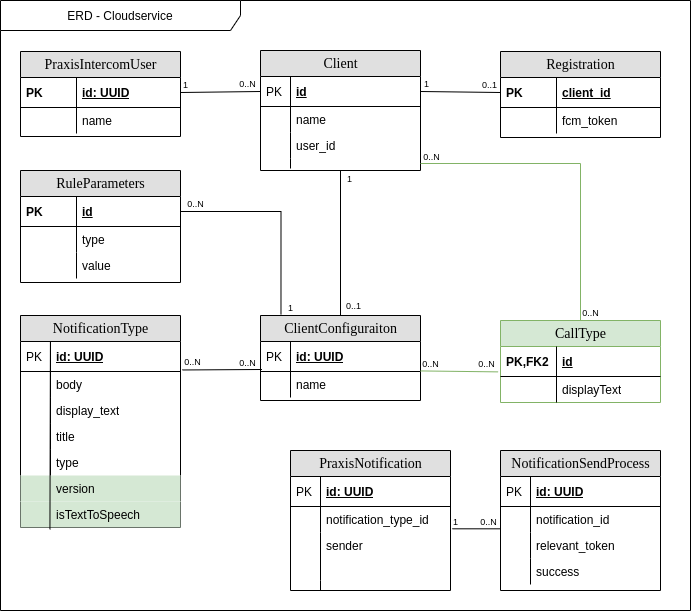
\includegraphics[width=\textwidth]{graphics/diagramms/erd_v02}}
        \caption{Entitiy Relation Diagramm - Cloudservice}
    \end{minipage}
\end{figure}

\clearpage
